\documentclass[11pt,a4paper]{article}

\usepackage{fontspec}
\setmainfont{Times New Roman}
\usepackage[a4paper,margin=2.5cm]{geometry}
\usepackage{microtype}
\usepackage{setspace}
\setstretch{1.12}
\usepackage{amsmath,amssymb}
\usepackage{booktabs}
\usepackage{longtable}
\usepackage{graphicx}
\usepackage{float}
\usepackage{caption}
\usepackage{enumitem}
\usepackage{siunitx}
\usepackage[numbers,sort&compress]{natbib}
\usepackage{hyperref}

\graphicspath{{../../outputs/thesis/figures/}}
\hypersetup{
  colorlinks=true,
  linkcolor=black,
  citecolor=black,
  urlcolor=blue,
  pdftitle={Explainable carbon intensity of national power systems: OWID, 2000--2025}
}
\captionsetup{font=small,labelfont=bf}
\setlength{\parindent}{1.1cm}
\setlength{\parskip}{0.2em}
\setlist[itemize]{topsep=0.25em,itemsep=0.15em}
\setlength{\emergencystretch}{3em}

\title{\textbf{Mô hình hóa có khả năng giải thích cường độ carbon của hệ thống điện quốc gia: bằng chứng từ Our World in Data, 2000--2025}}
\author{[Bổ sung tên tác giả và đơn vị]}
\date{Tháng 10 năm 2026}

\begin{document}
\maketitle

\begin{abstract}
Cường độ carbon của điện khác biệt đáng kể giữa các quốc gia và biến động theo
cơ cấu nguồn phát. Nghiên cứu này xây dựng một quy trình học máy có khả năng
giải thích để mô hình hóa cường độ phát thải vòng đời của điện từ dữ liệu quốc
gia--năm trong giai đoạn 2000--2025. Dữ liệu được tải từ các endpoint OWID
Grapher và ghép thành panel gồm 5.267 quan sát thuộc 210 quốc gia. Sáu họ mô
hình được đánh giá bằng các giao thức tách theo thời gian, quốc gia chưa thấy
và chuyển giao vùng. CatBoost được lựa chọn chỉ bằng RMSE trên validation theo
thời gian; trên test 2022--2025, mô hình đạt MAE 24,68, RMSE 41,04
gCO$_2$e/kWh và $R^2=0,972$. Khi đánh giá trên các quốc gia chưa xuất hiện trong
train, RMSE tăng lên 110,61 và $R^2$ giảm còn 0,749. SHAP xếp tỷ trọng thủy
điện và than là hai đặc trưng có đóng góp tuyệt đối trung bình lớn nhất.
Nghiên cứu tình huống Việt Nam cho thấy dự báo năm 2025 cao hơn quan sát 70,69
gCO$_2$e/kWh; các kịch bản thay đổi cơ cấu nguồn chỉ được diễn giải là phản ứng
ceteris paribus của mô hình, không phải tác động nhân quả hay khuyến nghị quy
hoạch. Kết quả cho thấy boosting có hiệu năng nội suy theo thời gian cao, đồng
thời nhấn mạnh khoảng cách tổng quát hóa giữa quốc gia và giới hạn của dữ liệu
quốc gia theo năm.

\medskip
\noindent\textbf{Từ khóa:} cường độ carbon điện; cơ cấu nguồn điện; học máy giải
thích được; SHAP; CatBoost; Our World in Data.
\end{abstract}

\begin{abstract}
\noindent\textbf{Abstract.}
This study develops an explainable machine-learning workflow for modelling
the life-cycle carbon intensity of national electricity systems using
country--year data from Our World in Data (OWID), 2000--2025. The assembled
panel contains 5,267 observations from 210 countries. Six model families are
evaluated under temporal, unseen-country, and region-transfer protocols.
CatBoost is selected solely by temporal-validation RMSE and obtains a
2022--2025 test MAE of 24.68, RMSE of 41.04 gCO$_2$e/kWh, and
$R^2=0.972$. On countries excluded from training, its RMSE rises to 110.61
and $R^2$ falls to 0.749. SHAP ranks hydro and coal shares as the two most
important features by mean absolute contribution. The Vietnam case and
composition scenarios are model-based, ceteris-paribus analyses, not causal
estimates. The results indicate strong temporal interpolation but materially
weaker transfer to unseen countries, motivating cautious use of country-level
annual models.
\end{abstract}

\noindent\textbf{Keywords:} electricity carbon intensity; generation mix;
explainable machine learning; SHAP; CatBoost; Our World in Data.

\section{Giới thiệu}

Điện năng là đầu vào thiết yếu cho quá trình điện hóa giao thông, công nghiệp
và tòa nhà; vì vậy, phát thải gắn với mỗi đơn vị điện ảnh hưởng trực tiếp đến
lợi ích khí hậu của các hoạt động sử dụng điện. Cường độ carbon vòng đời bổ
sung các phát thải ngoài vận hành nhà máy vào phép đo, qua đó mở rộng cách nhìn
so với chỉ tính phát thải tại điểm phát điện \citep{owid_carbon,ember_method}.
Chỉ số này khác nhau lớn giữa các hệ thống điện, một phần do tỷ trọng than,
khí, dầu, thủy điện, hạt nhân, gió và mặt trời.

Quan hệ giữa cơ cấu nguồn điện và cường độ carbon có thể phi tuyến, đồng thời
các tỷ trọng là thành phần của một hỗn hợp có tổng bị ràng buộc. Mô hình tuyến
tính tạo đường cơ sở dễ đối chiếu, trong khi mô hình cây có thể nắm bắt tương
tác và ngưỡng nhưng cần đánh giá nghiêm ngặt ngoài mẫu và giải thích thận
trọng. Đặc biệt, phép chia ngẫu nhiên từng hàng của panel có thể đặt các năm
cùng quốc gia vào cả train và test, khiến hiệu năng có vẻ lạc quan khi mục
tiêu là áp dụng cho năm sau hoặc quốc gia mới.

Nghiên cứu đặt ra ba câu hỏi:
\begin{enumerate}[leftmargin=1.6em]
  \item Các mô hình học máy ước lượng cường độ carbon điện tốt đến mức nào
  trên các năm nằm ngoài giai đoạn huấn luyện?
  \item Hiệu năng có duy trì khi chuyển sang quốc gia hoặc vùng địa lý chưa
  xuất hiện trong train hay không?
  \item Những thành phần nào chi phối dự báo, và mô hình phản ứng ra sao trước
  các kịch bản thay đổi cơ cấu nguồn của Việt Nam?
\end{enumerate}

Đóng góp của bài viết là: (i) xây dựng panel tái lập từ nguồn OWID Grapher có
ghi nhận phiên bản và checksum; (ii) so sánh sáu họ mô hình dưới ba giao thức
đánh giá bổ sung cho nhau; và (iii) kết hợp SHAP, permutation importance,
partial dependence cùng phân tích tình huống Việt Nam. Toàn bộ kết quả XAI và
kịch bản được diễn giải như thuộc tính của hàm dự báo, không phải bằng chứng
nhân quả.

\section{Dữ liệu}

\subsection{Nguồn và đơn vị phân tích}

Đơn vị phân tích là một quốc gia trong một năm. Panel bao phủ 2000--2025, với
5.267 dòng sau quy tắc loại hàng quá thưa, thuộc 210 quốc gia và năm vùng địa
lý. Các đại lượng về phát điện theo nguồn, tổng sản lượng, nhu cầu, nhập khẩu
ròng, điện bình quân đầu người, dân số và GDP/người được lấy từ CSV API của
OWID Grapher. Biến đích cường độ carbon được lấy từ cùng Grapher với metric
\texttt{carbon\_intensity}; OWID ghi nguồn Ember cho chuỗi này
\citep{owid_carbon,owid_electricity,ember_method}.

Biến đích là cường độ phát thải vòng đời, đơn vị
gCO$_2$e/kWh. Phạm vi mô hình chính giới hạn ở thực thể quốc gia có mã ISO;
Kosovo được giữ lại theo mã OWID riêng. Các tổng hợp khu vực và toàn cầu bị
loại. Panel giữ các tỷ trọng nguồn điện, quy mô phát điện và nhu cầu, nhập
khẩu ròng, dân số, GDP và điện bình quân đầu người để kiểm tra và mô tả dữ
liệu. Dữ liệu GDP/người, phát điện tổng, điện bình quân đầu người và tổng tỷ
trọng tái tạo không được dùng trong ma trận đặc trưng cuối cùng do thiếu hụt
hoặc dư thừa đại số với các biến khác.

\subsection{Đặc trưng và kiểm soát chất lượng}

Tỷ trọng mỗi nguồn được tính bằng sản lượng của nguồn chia tổng sản lượng
điện. Tỷ lệ nhập khẩu ròng được tính bằng nhập khẩu ròng chia nhu cầu. Mỗi hàng
cần ít nhất 9 trong 11 trường đầu vào thô bắt buộc; 120 hàng không đáp ứng
điều kiện này bị loại khỏi 5.387 hàng ban đầu. Các giá trị thiếu còn lại được
điền bằng median được ước lượng bên trong pipeline trên phần train của từng
fold, tránh học thông tin từ validation hoặc test.

Ma trận mô hình gồm 11 đặc trưng: tỷ trọng than, khí, mặt trời, gió, thủy
điện, hạt nhân và nhiên liệu sinh học; $\log(1+\text{nhu cầu điện})$;
tỷ trọng nhập khẩu ròng trên nhu cầu; $\log(1+\text{dân số})$; và xu thế năm
tính từ 2000. Tỷ trọng dầu là thành phần tham chiếu không đưa trực tiếp vào
ma trận, do tổng các tỷ trọng nguồn bị ràng buộc. Việc chọn thành phần tham
chiếu được kiểm tra bằng VIF trên train; lựa chọn bỏ dầu cho VIF tối đa thấp
nhất trong các lựa chọn đã xét.

\section{Phương pháp}

\subsection{Mô hình dự báo}

Với quốc gia $i$ ở năm $t$, bài toán được viết:
\begin{equation}
  y_{it}=f(\mathbf{x}_{it})+\varepsilon_{it},
\end{equation}
trong đó $y_{it}$ là cường độ carbon và $\mathbf{x}_{it}$ là vector 11 đặc
trưng. Sáu họ mô hình được so sánh: Linear Regression, Ridge, Elastic Net,
Random Forest, XGBoost và CatBoost. Ridge và Elastic Net cung cấp các baseline
tuyến tính có điều chuẩn \citep{hoerl1970,zou2005}; Random Forest kết hợp
nhiều cây quyết định \citep{breiman2001}; XGBoost và CatBoost là các phương
pháp boosting cây cho dữ liệu bảng \citep{chen2016,prokhorenkova2018}.

Các pipeline xử lý giá trị thiếu được fit trong từng tập huấn luyện; biến
chuẩn hóa chỉ được áp dụng cho các mô hình tuyến tính. Siêu tham số được chọn
theo RMSE validation. Với giao thức thời gian, CatBoost có cấu hình depth 6,
800 vòng lặp và learning rate 0,05; RMSE validation là 39,94 gCO$_2$e/kWh.
Sau khi chọn cấu hình, mô hình được fit lại trên train cộng validation và chỉ
sau đó đánh giá trên test.

\subsection{Giao thức đánh giá}

Ba giao thức kiểm tra các dạng tổng quát hóa khác nhau:
\begin{itemize}
  \item \textbf{Theo thời gian:} train 2000--2018 (3.943 dòng), validation
  2019--2021 (627 dòng), test 2022--2025 (697 dòng). Không năm nào đồng thời
  xuất hiện ở nhiều split.
  \item \textbf{Quốc gia chưa thấy:} các quốc gia được phân hoạch độc quyền
  theo tỷ lệ 60/20/20 với seed 42. Test gồm 42 quốc gia và 1.047 quan sát;
  không quốc gia nào xuất hiện trong train hoặc validation.
  \item \textbf{Chuyển giao vùng:} lần lượt giữ lại Africa, America, Asia,
  Europe hoặc Oceania; huấn luyện trên các vùng còn lại đến năm 2021 và kiểm
  tra trên vùng giữ lại trong 2022--2025.
\end{itemize}

Hiệu năng được báo cáo bằng MAE, RMSE và hệ số xác định:
\begin{align}
  \mathrm{MAE} &= \frac{1}{n}\sum_{j=1}^{n}|y_j-\hat y_j|,\\
  \mathrm{RMSE} &= \sqrt{\frac{1}{n}\sum_{j=1}^{n}(y_j-\hat y_j)^2},\\
  R^2 &= 1-\frac{\sum_{j=1}^{n}(y_j-\hat y_j)^2}
                  {\sum_{j=1}^{n}(y_j-\bar y)^2}.
\end{align}
Đơn vị MAE và RMSE là gCO$_2$e/kWh. Seed cố định bằng 42. Các metric test
không được sử dụng để chọn mô hình hoặc siêu tham số.

\subsection{Giải thích và kịch bản}

SHAP phân rã dự báo thành đóng góp đặc trưng dựa trên giá trị Shapley
\citep{lundberg2017}. Permutation importance đánh giá mức suy giảm dự báo khi
hoán vị một đặc trưng; partial dependence mô tả đáp ứng trung bình của mô hình
theo một đặc trưng. Vì các thành phần cơ cấu điện tương quan và có quan hệ
thành phần, các phương pháp này mô tả mô hình đã fit chứ không nhận diện tác
động độc lập hay quan hệ nhân quả.

Các kịch bản Việt Nam bắt đầu từ cấu hình quan sát năm 2025. Tỷ trọng nguồn
được điều chỉnh theo tên kịch bản, trong khi nhu cầu, dân số, nhập khẩu và năm
được giữ cố định. Mỗi thay đổi là một phản thực ceteris paribus trong không
gian đầu vào của mô hình, không phải dự báo cân bằng hệ thống điện hay đánh
giá chính sách.

\section{Kết quả}

\subsection{Đánh giá ngoài mẫu}

CatBoost được chọn dựa trên RMSE validation theo thời gian. Trên temporal
test, mô hình đạt MAE 24,68, RMSE 41,04 gCO$_2$e/kWh và $R^2=0,972$. Đây là
kết quả tốt nhất trong sáu mô hình theo temporal test, nhưng khoảng cách giữa
validation và test cùng với sự thay đổi thành phần quốc gia theo năm gần nhất
cần được tính đến khi diễn giải. Trên giao thức quốc gia chưa thấy, cùng mô
hình đạt MAE 60,70, RMSE 110,61 và $R^2=0,749$.

\begin{table}[H]
\centering
\caption{Hiệu năng của sáu mô hình trên temporal test và unseen-country test.}
\label{tab:model_metrics}
\small
\begin{tabular}{llrrr}
\toprule
Giao thức & Mô hình & MAE & RMSE & $R^2$\\
\midrule
\multicolumn{5}{l}{\textit{Temporal test (2022--2025), $n=697$}}\\
& Linear Regression & 49,75 & 82,78 & 0,887\\
& Ridge & 49,75 & 82,78 & 0,887\\
& Elastic Net & 49,73 & 82,78 & 0,887\\
& Random Forest & 30,70 & 49,05 & 0,960\\
& XGBoost & 27,72 & 47,69 & 0,962\\
& CatBoost & \textbf{24,68} & \textbf{41,04} & \textbf{0,972}\\
\midrule
\multicolumn{5}{l}{\textit{Unseen-country test, $n=1.047$}}\\
& Linear Regression & 61,06 & 100,59 & 0,792\\
& Ridge & 60,82 & 100,53 & 0,792\\
& Elastic Net & 60,27 & 100,38 & 0,793\\
& Random Forest & 65,32 & 115,55 & 0,726\\
& XGBoost & 59,49 & 107,07 & 0,764\\
& CatBoost & 60,70 & 110,61 & 0,749\\
\bottomrule
\end{tabular}
\end{table}

Hiệu năng unseen-country của CatBoost kém hơn rõ rệt so với temporal test,
đặc biệt theo RMSE. Trong giao thức unseen-country, Elastic Net có RMSE thấp
nhất trong sáu mô hình (100,38) và $R^2$ cao nhất (0,793), cho thấy mô hình
phi tuyến được chọn cho nội suy thời gian không đương nhiên tối ưu cho chuyển
giao quốc gia. Kết quả này là lý do cần báo cáo nhiều hơn một cách chia dữ
liệu.

\begin{figure}[H]
\centering
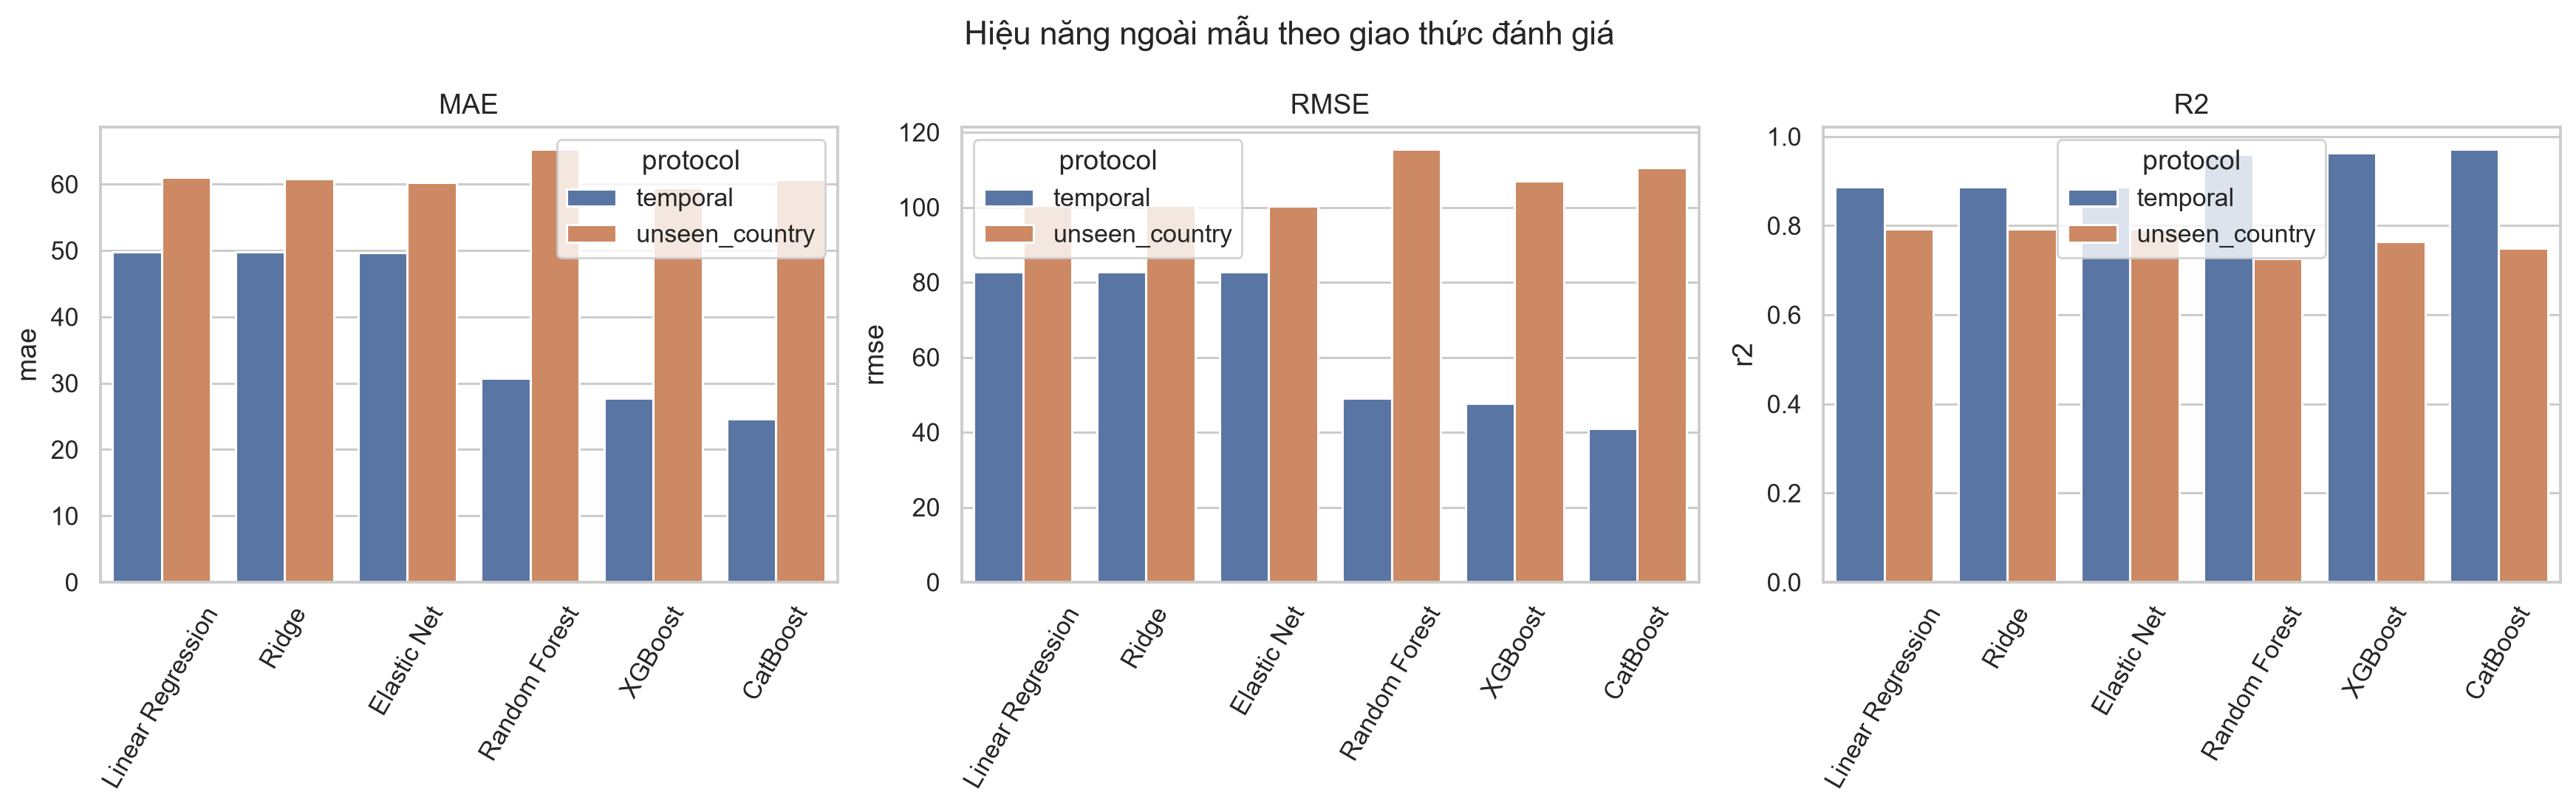
\includegraphics[width=0.9\textwidth]{model_comparison.png}
\caption{So sánh hiệu năng mô hình trên temporal và unseen-country test.}
\label{fig:model_comparison}
\end{figure}

\subsection{Chuyển giao giữa các vùng}

\begin{table}[H]
\centering
\caption{RMSE CatBoost khi giữ lại từng vùng địa lý.}
\label{tab:region_transfer}
\begin{tabular}{lrr}
\toprule
Vùng giữ lại & Số quan sát test & RMSE (gCO$_2$e/kWh)\\
\midrule
Africa & 168 & 72,803\\
America & 147 & 40,185\\
Asia & 176 & 133,880\\
Europe & 160 & 144,124\\
Oceania & 46 & 107,399\\
\bottomrule
\end{tabular}
\end{table}

Sai số chuyển giao dao động đáng kể theo vùng: RMSE thấp nhất ở America và cao
nhất ở Europe. CatBoost không phải mô hình tốt nhất ở mọi lần giữ vùng; các
mô hình tuyến tính có RMSE thấp hơn ở Europe và Oceania. Việc giữ cả vùng ra
khỏi train là phép thử ngoại suy cấu trúc nghiêm ngặt hơn phép chia thời gian
trong cùng panel. Do đó, kết quả này không nên được thay thế bằng một điểm
hiệu năng tổng hợp duy nhất.

\begin{figure}[H]
\centering
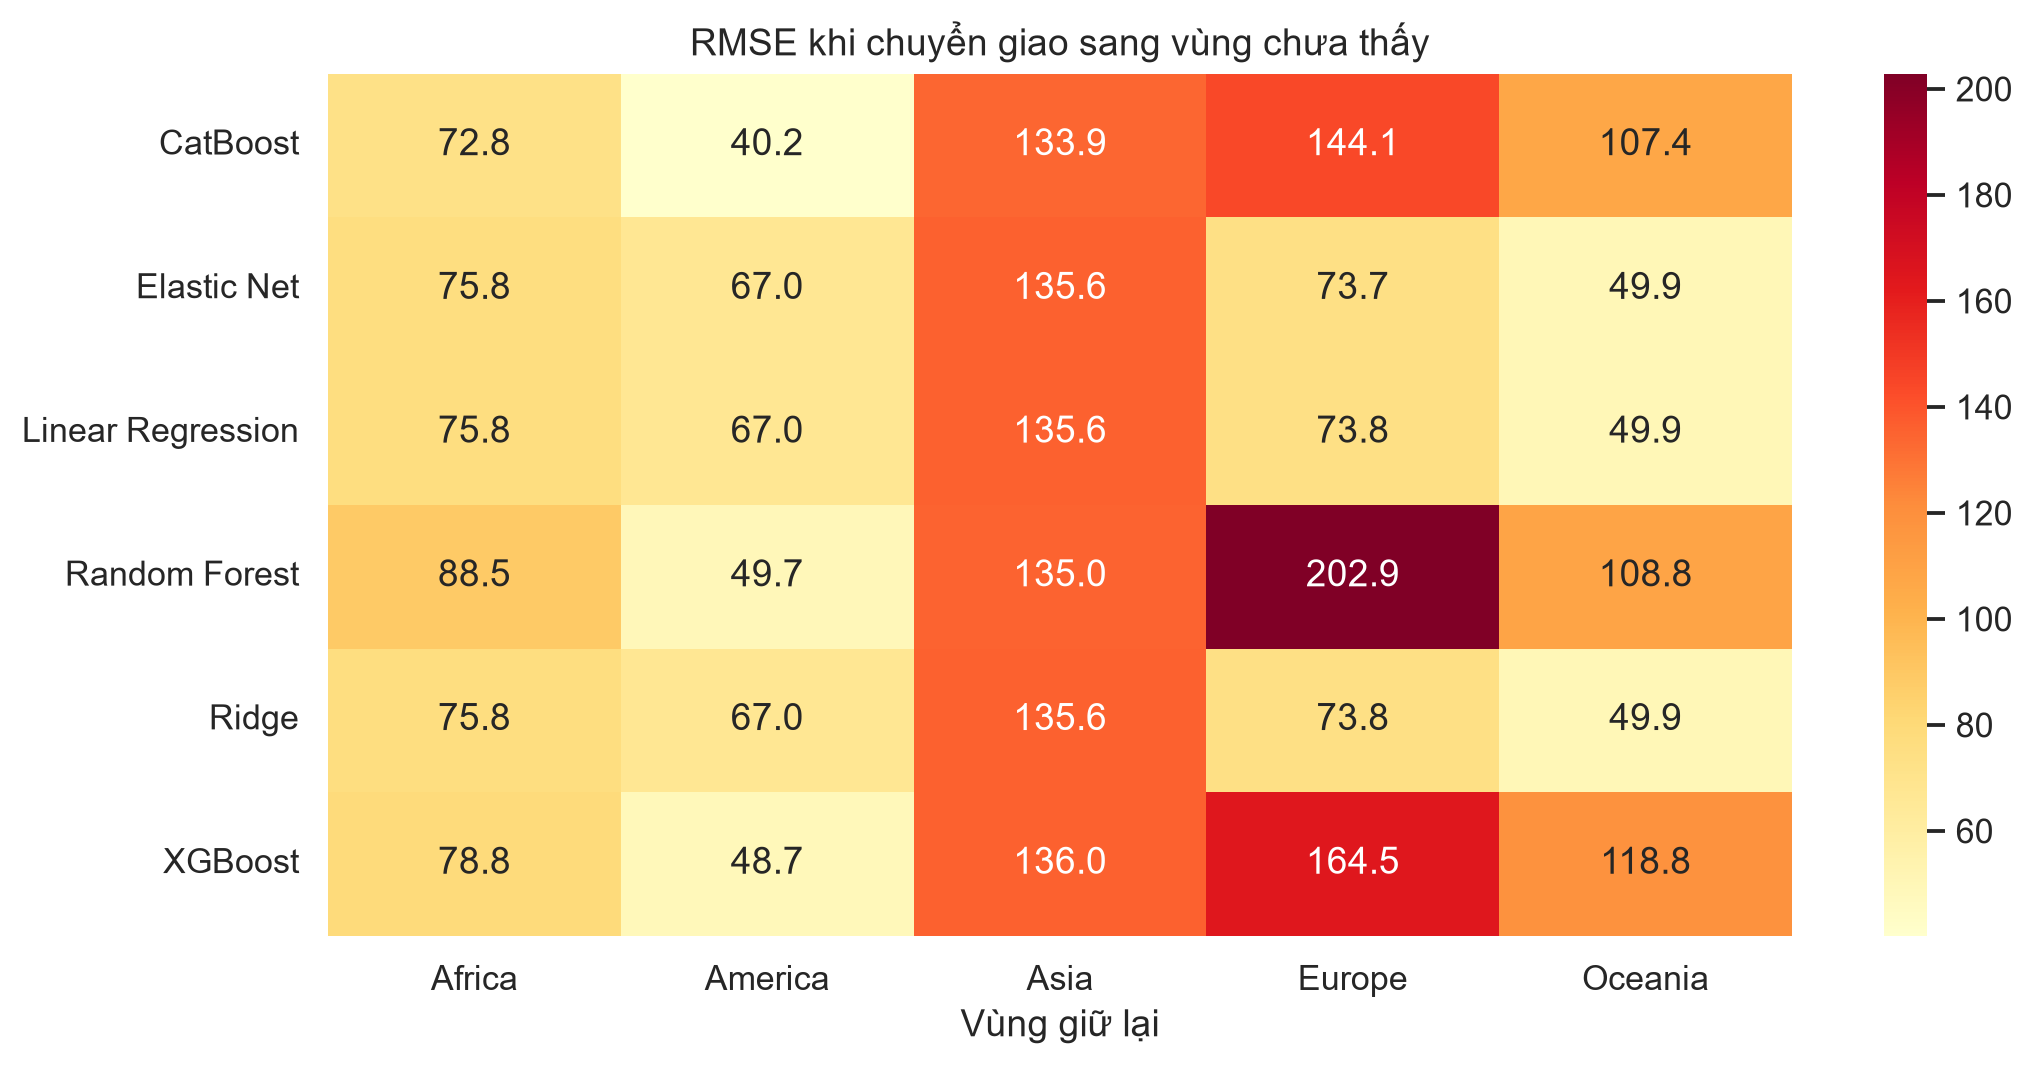
\includegraphics[width=0.88\textwidth]{region_transfer_rmse.png}
\caption{RMSE theo vùng được giữ lại trong giao thức chuyển giao vùng.}
\label{fig:region_transfer}
\end{figure}

\subsection{Giải thích mô hình}

Tỷ trọng thủy điện có mean absolute SHAP lớn nhất (140,68 gCO$_2$e/kWh),
tiếp theo là than (47,90), gió (34,63), hạt nhân (33,17) và nhiên liệu sinh
học (25,63). Chênh lệch lớn của thủy điện phản ánh vai trò nổi bật của đặc
trưng này trong các dự báo trên phân phối dữ liệu đã quan sát. Nó không có
nghĩa một thay đổi thủy điện độc lập sẽ gây ra mức giảm/tăng tương ứng: SHAP
chịu ảnh hưởng của quan hệ tương quan, thành phần và các biến không quan sát.

\begin{table}[H]
\centering
\caption{Năm đặc trưng đứng đầu theo mean absolute SHAP của CatBoost.}
\label{tab:shap}
\begin{tabular}{lrr}
\toprule
Đặc trưng & Mean $|\mathrm{SHAP}|$ & Mean SHAP\\
\midrule
Tỷ trọng thủy điện & 140,68 & 9,73\\
Tỷ trọng than & 47,90 & -4,62\\
Tỷ trọng điện gió & 34,63 & -21,44\\
Tỷ trọng hạt nhân & 33,17 & -2,47\\
Tỷ trọng nhiên liệu sinh học & 25,63 & -8,45\\
\bottomrule
\end{tabular}
\end{table}

\begin{figure}[H]
\centering
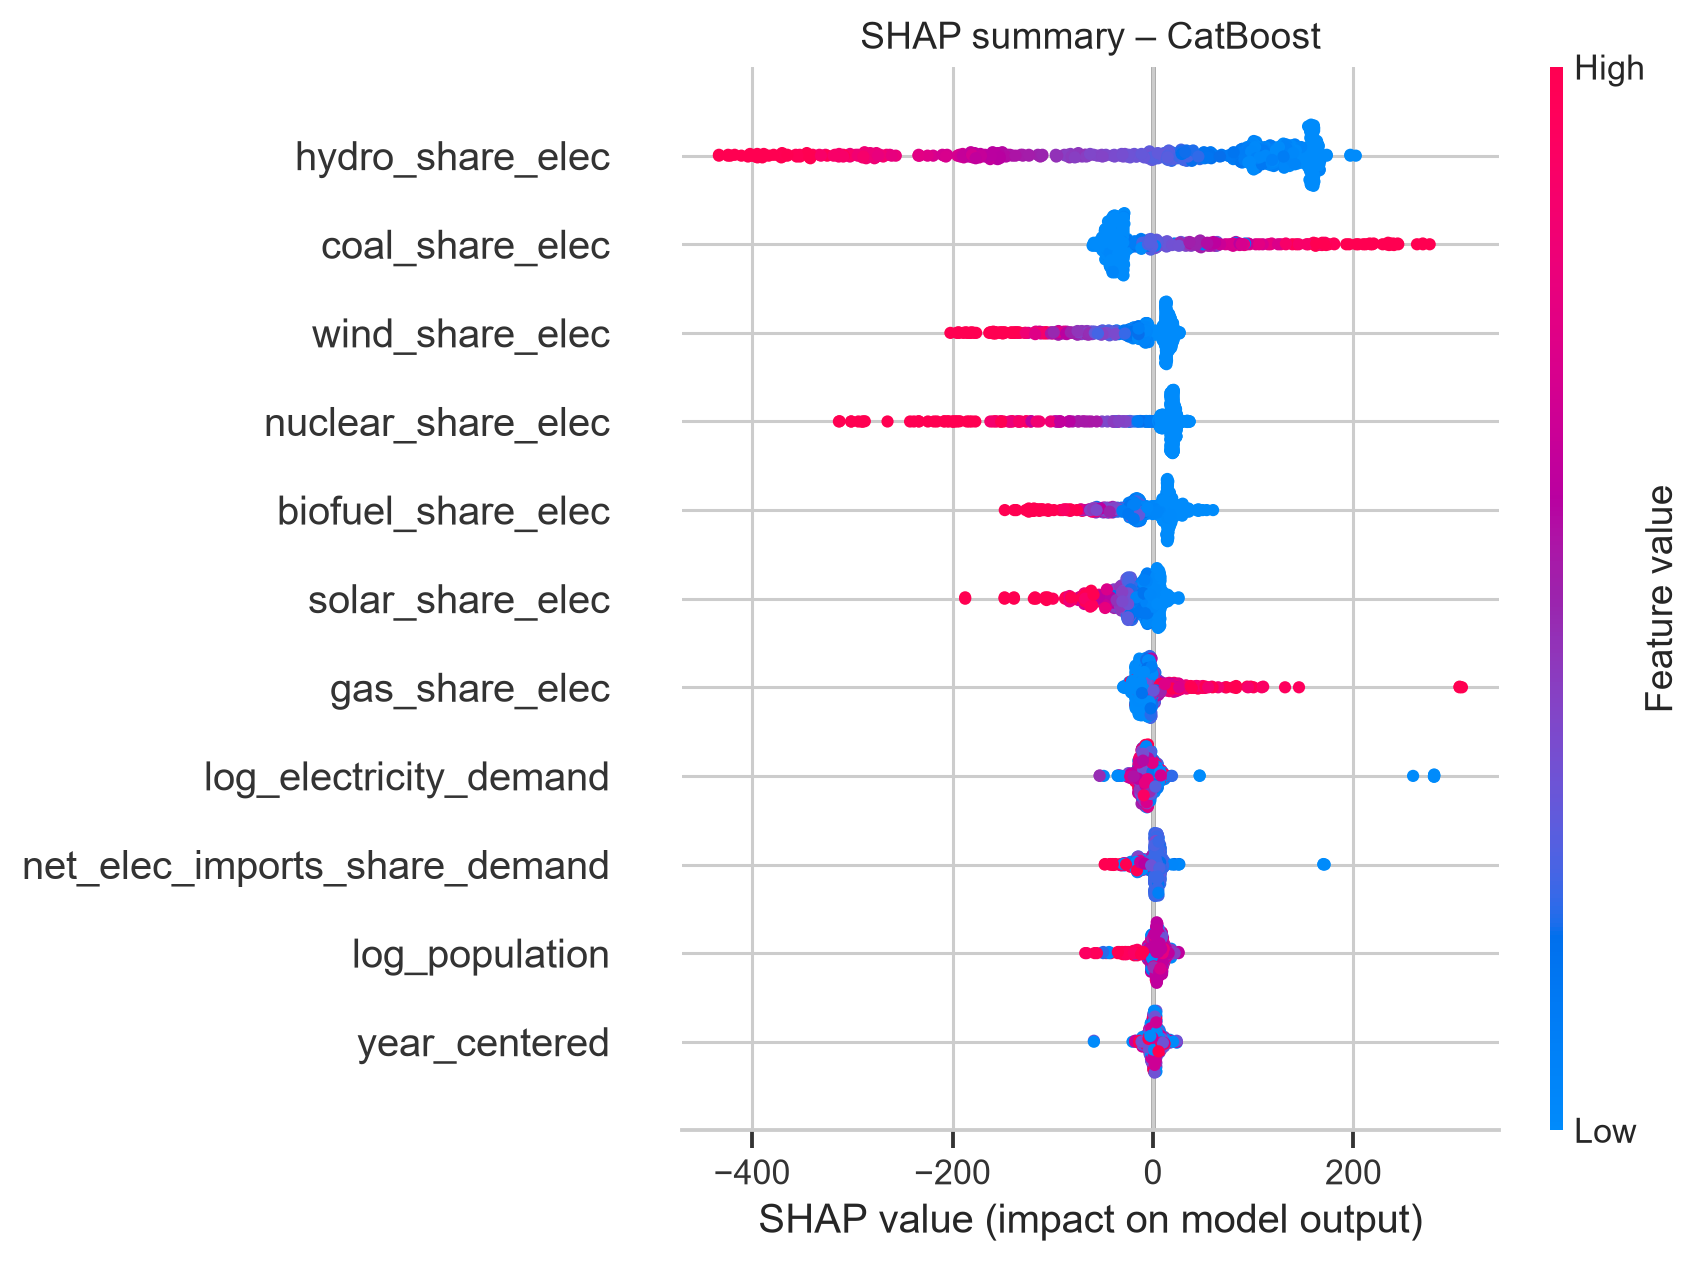
\includegraphics[width=0.94\textwidth]{shap_summary.png}
\caption{Phân bố đóng góp SHAP của mô hình CatBoost trên mẫu giải thích.}
\label{fig:shap_summary}
\end{figure}

Permutation importance và partial dependence được dùng như các góc nhìn bổ
sung cho SHAP. Sự phù hợp giữa các phương pháp có thể củng cố mô tả về hàm dự
báo, nhưng không loại bỏ vấn đề phụ thuộc giữa các tỷ trọng nguồn. Hình
partial dependence vì vậy cần được đọc như đáp ứng trung bình trong miền dữ
liệu, không như kết quả của một can thiệp khả thi trong vận hành hệ thống.

\subsection{Nghiên cứu tình huống Việt Nam}

Trong dữ liệu OWID năm 2025, cường độ carbon quan sát của Việt Nam là 460,73
gCO$_2$e/kWh; dự báo CatBoost là 531,42, tương ứng sai số dự báo dương 70,69.
Kết quả cá biệt này cho thấy hiệu năng toàn cục cao không đảm bảo độ chính
xác tương đương cho từng quốc gia hoặc từng năm.

\begin{table}[H]
\centering
\caption{Các kịch bản cơ cấu nguồn điện giả định cho Việt Nam năm 2025.}
\label{tab:vietnam_scenarios}
\small
\begin{tabular}{p{6.2cm}rrr}
\toprule
Kịch bản & Dự báo & Thay đổi & Thay đổi (\%)\\
 & (gCO$_2$e/kWh) & (gCO$_2$e/kWh) & \\
\midrule
Quan sát cơ sở & 531,42 & 0,00 & 0,00\\
Mặt trời +5 điểm, than -5 điểm & 482,85 & -48,57 & -9,14\\
Gió +5 điểm, than -5 điểm & 470,29 & -61,13 & -11,50\\
Mặt trời +5, gió +5, than -10 điểm & 427,48 & -103,94 & -19,56\\
Hạt nhân +5 điểm, than -5 điểm & 470,57 & -60,86 & -11,45\\
Thủy điện -5 điểm, khí +5 điểm & 573,88 & 42,46 & 7,99\\
\bottomrule
\end{tabular}
\end{table}

Trong các cấu hình được kiểm tra, kịch bản tăng 5 điểm phần trăm mặt trời và
5 điểm gió, đồng thời giảm 10 điểm than, tạo mức giảm dự báo lớn nhất
(103,94 gCO$_2$e/kWh). Kịch bản thay 5 điểm thủy điện bằng khí làm dự báo tăng
42,46. Đây là chênh lệch đầu ra khi giữ các biến khác cố định; phép thử không
mô hình hóa tính khả thi về lưới điện, công suất dự phòng, lưu trữ, chi phí,
an ninh cung cấp hay đáp ứng nhu cầu.

\begin{figure}[H]
\centering
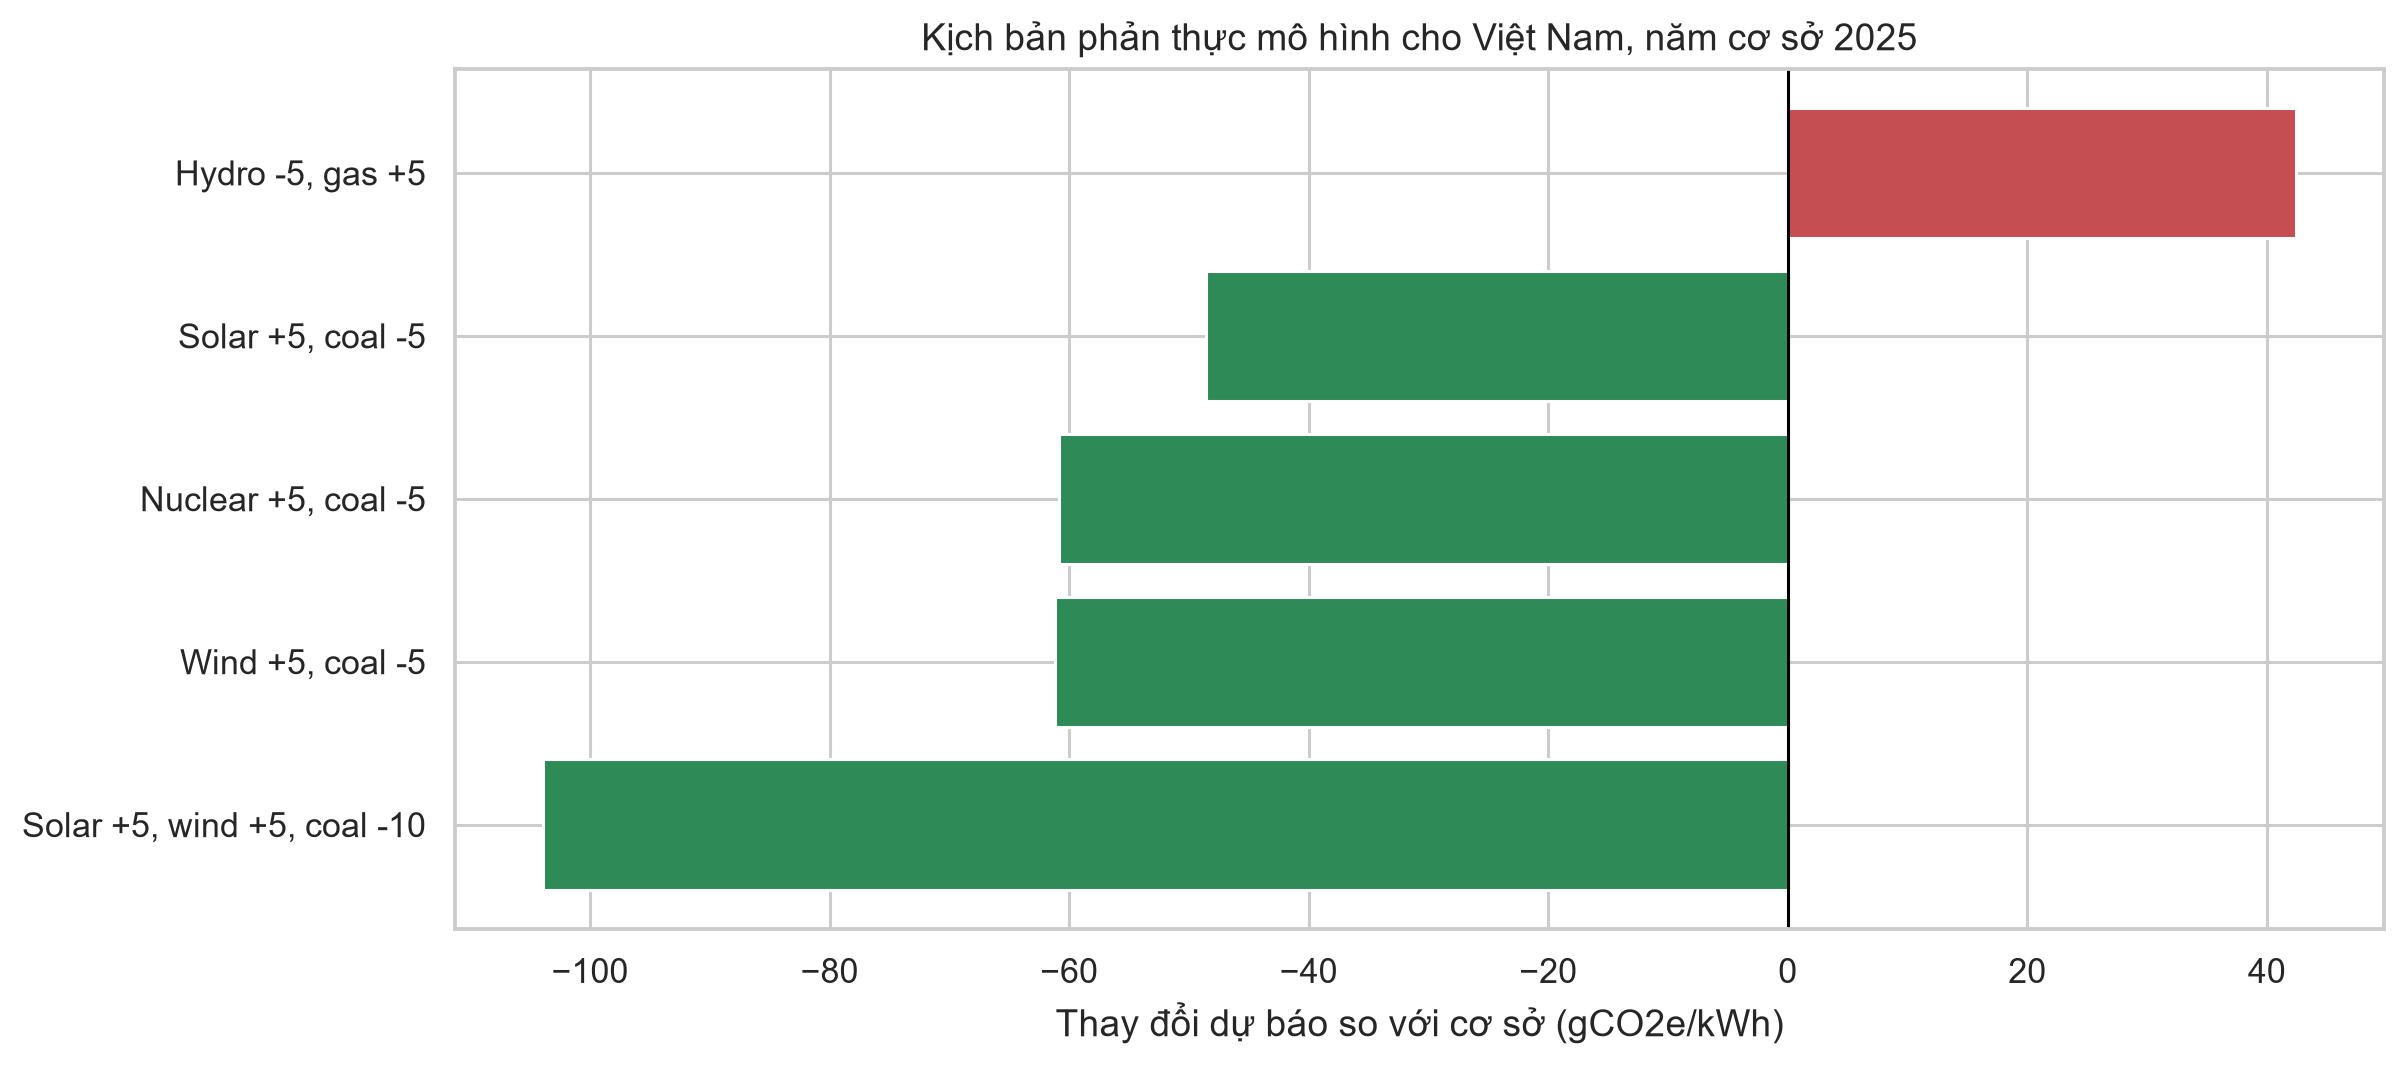
\includegraphics[width=0.88\textwidth]{vietnam_scenarios.png}
\caption{Dự báo CatBoost trong các kịch bản thay đổi tỷ trọng nguồn điện của Việt Nam.}
\label{fig:vietnam_scenarios}
\end{figure}

\section{Thảo luận}

Kết quả cho thấy mô hình boosting cây biểu diễn tốt dữ liệu theo thời gian khi
các quốc gia đã xuất hiện trong tập huấn luyện. Lợi thế của CatBoost trước các
mô hình tuyến tính và các boosting khác trên temporal test phù hợp với giả
thuyết về quan hệ phi tuyến và tương tác giữa cơ cấu nguồn và cường độ carbon.
Tuy nhiên, giảm hiệu năng trên unseen-country test và độ biến thiên lớn trong
region-transfer cho thấy chất lượng nội suy không thể được xem là bằng chứng
cho khả năng chuyển giao phổ quát.

Một nguyên nhân quan trọng là đặc trưng và biến đích đều được đo trong cùng
năm. Vì vậy, bài toán chính là mô hình hóa hoặc nowcasting có điều kiện trên
cơ cấu điện hiện thời, không phải dự báo nhiều năm trước khi biết cơ cấu đó.
Nếu mục tiêu là dự báo tương lai, cần dự báo hoặc quy định ngoại sinh các biến
đầu vào như cơ cấu nguồn, nhu cầu và nhập khẩu, rồi đánh giá toàn bộ chuỗi dự
báo theo thiết kế riêng.

Các kết quả SHAP và kịch bản có thể hỗ trợ kiểm tra tính hợp lý của dự báo,
phát hiện trường hợp cần xem xét và khảo sát độ nhạy cục bộ. Chúng không thay
thế phân tích nhân quả hoặc mô hình tối ưu hóa hệ thống điện. Đặc biệt, tính
thành phần của tỷ trọng nguồn khiến việc thay đổi một thành phần trong khi
không cân đối thành phần còn lại có thể tạo điểm nằm ngoài miền dữ liệu thực.

\subsection{Hạn chế}

\begin{enumerate}[leftmargin=1.6em]
  \item Dữ liệu theo năm ở cấp quốc gia che lấp khác biệt theo giờ, vùng lưới,
  công nghệ và cấu trúc vận hành.
  \item Các số liệu OWID có thể được cập nhật hồi tố; độ phủ năm 2025 chưa
  đồng nhất giữa các quốc gia. Vì thế, khả năng tái lập chính xác đòi hỏi lưu
  lại snapshot nguồn và checksum đi kèm lần chạy.
  \item Bổ sung median giúp pipeline xử lý dữ liệu thiếu nhưng không khắc
  phục thiên lệch nếu thiếu dữ liệu có hệ thống.
  \item SHAP, permutation importance và partial dependence chịu ảnh hưởng bởi
  tương quan và phân phối quan sát; chúng không nhận dạng hiệu ứng nhân quả.
  \item Kịch bản Việt Nam giữ các biến khác không đổi và không áp đặt ràng
  buộc kỹ thuật, kinh tế hoặc chính sách của hệ thống điện.
\end{enumerate}

\section{Kết luận}

Bài viết xây dựng và đánh giá một quy trình học máy có khả năng giải thích cho
cường độ carbon vòng đời của điện quốc gia trong giai đoạn 2000--2025. Trên
panel 5.267 quan sát thuộc 210 quốc gia, CatBoost đạt RMSE 41,04
gCO$_2$e/kWh trên temporal test, nhưng RMSE tăng lên 110,61 khi đánh giá trên
các quốc gia chưa thấy. SHAP xác định tỷ trọng thủy điện và than là hai đặc
trưng có đóng góp tuyệt đối trung bình lớn nhất trong mô hình được chọn.
Kịch bản Việt Nam cho thấy dự báo nhạy với các thay đổi tỷ trọng nguồn, song
không thể diễn giải thành tác động chính sách.

Kết luận thực tiễn là mô hình có ích cho mô hình hóa có điều kiện, so sánh và
thăm dò độ nhạy trong phạm vi dữ liệu đã quan sát. Trước khi dùng để lập kế
hoạch hoặc chuyển giao sang quốc gia mới, cần kiểm định ngoài mẫu phù hợp,
định lượng bất định và tích hợp mô hình hệ thống điện với các ràng buộc vận
hành. Hướng tiếp theo gồm backtesting qua nhiều cửa sổ thời gian, dữ liệu có
tần suất cao hơn, mô hình phân cấp theo quốc gia/vùng và thiết kế nhận dạng
nhân quả cho câu hỏi chính sách.

\section*{Khả năng tái lập và nguồn dữ liệu}

Notebook thực nghiệm và mã nguồn nằm trong repository dự án. Các bảng kết
quả, dự báo, hình, mô hình đã fit, audit dữ liệu và manifest chạy được lưu
dưới \texttt{outputs/thesis/}. Lần chạy ghi lại seed, phiên bản thư viện, URL
nguồn và SHA-256 của các tệp tải về. Do OWID Grapher có thể được cập nhật,
các con số trong bài gắn với snapshot đã lưu trong artifact, không nhất thiết
trùng một lần tải dữ liệu mới trong tương lai.

\bibliographystyle{plainnat}
\bibliography{references}

\end{document}
